
%%%%%%%%%%%%%%%%%%%%%%% file typeinst.tex %%%%%%%%%%%%%%%%%%%%%%%%%
%
% This is the LaTeX source for the instructions to authors using
% the LaTeX document class 'llncs.cls' for contributions to
% the Lecture Notes in Computer Sciences series.
% http://www.springer.com/lncs       Springer Heidelberg 2006/05/04
%
% It may be used as a template for your own input - copy it
% to a new file with a new name and use it as the basis
% for your article.
%
% NB: the document class 'llncs' has its own and detailed documentation, see
% ftp://ftp.springer.de/data/pubftp/pub/tex/latex/llncs/latex2e/llncsdoc.pdf
%
%%%%%%%%%%%%%%%%%%%%%%%%%%%%%%%%%%%%%%%%%%%%%%%%%%%%%%%%%%%%%%%%%%%


%\documentclass[french,runningheads,a4paper]{llncs}
\documentclass[francais,a4paper]{llncs} % ou autre classe

\usepackage[utf8]{inputenc}
\usepackage[T1]{fontenc}
\usepackage{lmodern} % ou toute autre fonte complète pour le français : kpfonts, fourier...
\usepackage{xspace} % pour profiter du mécanisme
\usepackage[np]{numprint} % si je dois écrire des nombres sans unités sinon 
% \usepackage{siunitx} % si je dois écrire des grandeurs avec unités
%\usepackage[main=french]{babel}

\usepackage{amssymb}
\setcounter{tocdepth}{3}
\usepackage{graphicx}

\usepackage{url}

\newcommand{\keywords}[1]{\par\addvspace\baselineskip
\noindent\keywordname\enspace\ignorespaces#1}

%\mainmatter  % start of an individual contribution

% first the title is needed
\title{Évaluation des apports d'un reseau de neurones antagoniste pour une classification semi-supervisé de textes français issue d'une base de données faiblement labellisés}

% a short form should be given in case it is too long for the running head
\titlerunning{Apports d'un GAN pour une classification semi-supervisé}

% the name(s) of the author(s) follow(s) next
%
% NB: Chinese authors should write their first names(s) in front of
% their surnames. This ensures that the names appear correctly in
% the running heads and the author index.
%
\author{Dylan Baptiste \and Stéphane Cormier \and Shufan Jiang}
%
\authorrunning{Apports d'un GAN dans une classification semi-supervisé}
% (feature abused for this document to repeat the title also on left hand pages)

% the affiliations are given next; don't give your e-mail address
% unless you accept that it will be published
\institute{Université de Reims Champagne-Ardenne\\
dylan.baptiste@etudiant.univ-reims.fr\\
stephane.cormier@univ-reims.fr\\
shufan.jiang@univ-reims.fr\\}

%
% NB: a more complex sample for affiliations and the mapping to the
% corresponding authors can be found in the file "llncs.dem"
% (search for the string "\mainmatter" where a contribution starts).
% "llncs.dem" accompanies the document class "llncs.cls".
%

%\toctitle{test}
%\tocauthor{}
\setcounter{tocdepth}{3}

\graphicspath{ {../src/} }


\begin{document}

\let\oldaddcontentsline\addcontentsline
\def\addcontentsline#1#2#3{}
\maketitle
\def\addcontentsline#1#2#3{\oldaddcontentsline{#1}{#2}{#3}}

\begin{abstract}
Les tâches de classifications de textes se heurtent souvent au problème de bases de données peu voir pas labellisé. Ici nous nous intéressons au apports de l'ajout d'un GAN afin d'artificiellement créer des données labellisés. Le but est d'améliorer les performances d'un classifieur qui ne se serait entraîné que sur des données labellisé issue d'une petite base de données.
\keywords{réseau de neurones, réseaux antagonistes génératifs, traitement du language, classification, semi-supervisé}
\end{abstract}

\tableofcontents

\listoffigures

\listoftables

\section{Contexte}
Ce travail à été réalisé dans le cadre d'un TER (Travail d'Étude et de Recherche) par Dylan Baptiste, étudiant en 2 année de Master, supervisé par Shufan Jiang, doctorante, et Stéphane Cormier, enseignant-chercheur, à l'Université de Reims Champagne-Ardenne.

presentation des données\dots

\section{État de l'art}

	\subsection{Représentations d'encodeur bidirectionnel à partir de transformateurs (BERT)}
	Les modeles BERT (de l'anglais Bidirectional Encoder Representations from Transformers) sont des modeles de traintement du language introduit en 2018 par Google (TODO citer https://arxiv.org/abs/1810.04805) qui ont permis des ameliorations significatives dans ce domaine. BERT à été entrainé sur un copus de plusieurs langues. L'entrainement des modeles BERT s'effectue en deux etapes, tout d'abord une tache semi supervisé où des mots caviardé dans un texte doivent etre retrouvé par le modeles et une seconde supervisé où le modele doit determiner si une phrase B est la suite d'une phrase A ou non (Next-Sentence Prediction).
	CamemBERT est un modele basé sur la meme architecture mais entrainé uniquement sur un corpus francais où la tache (Next-Sentence Prediction) n'a pas été realisé.
	De tel modeles prennent en entrée des phrases encodées, pour chaque token dans la phrases encodées le modele produit en sortie un vecteur (de dimention 768 pour BERT et CamemBERT) et un autre vecteur (toujours de taille 768) pour l'ensempble de la sequence, token est appelé [CLS] et sa represneation en sortie est une represnetation dans l'espace, selon le modele, de la sequence encodé. C'est sur le token [CLS] que le modele est entrainé pour la tache de classification supervisé.
	(TODO image de BERT)
	
	\subsection{Réseaux antagonistes génératifs}
	Les GAN (de l'anglais Generative Adversarial Networks) sont une famille de reseau de neuronnes communement separable en deux partie antagonistes: un générateur (G) et un discriminateur (D) qui s'affornte lors de l'entrainement.
	Le generateur à pour but de generer des données sembalable à des donnée reel. Les applications les plus connus concerne la generation d'images (TODO: CITER ). Pour effectuer une telle tache ce model est adjoint à un autre modele appelé Discriminateur qui doit determiner si une données est reel (issue d'une base de données) ou genereré (c-a-d produite par le genrateur), il effectue donc une classification binaire.
	Il existe une multitude de variante de reseau antagoniste génératif notament les Conditional GAN (CGAN) dont la generation du G est conditionné par un ou des label.
	Dans ce travail c'est une sorte de CGAN qui sera utilisé.


\section{Données}
Les données qui servirons d'entrainement pour ce projet sont des messages francais issue du reseau social twitter. Certain message sont des observations d'agriculteur tandis que d'autre non. Les données sont donc labellisé binairement sur cette caracteristique. Nous disposons d'une base de donnée de XXX messages labelisé à la main: (TODO: donner les stats) XXX observation et XXX non observation, ainsi que XXX messages non labellisés.
\subsection{Extraction de caractéristiques}
Dans ce travaille il n'est pas question d'effectuer un entrainement de la partie du modele CamemBERT. Il y a donc une phase d'extraction des caracteristiques affin de limiter le temps de calcule lors des entrainements.
C'est dans cette phase que l'on doit choisir quelles sorties de CamemBERT utiliser pour la representation des message.
Pour ce travail seul l'encodage du token [CLS] est utilisé. Ce choix arbitraire ouvre des prespetive de travail qui seront discuté dans la derniere partie. 
Chaque message est donc à present "vectoriser" dans un espace de 768 dimentions. Les label associé aux messages annotés manuellement sont reporté aux vecteurs associé au message et les vecteurs des messages non labellisés reste non labellisés 

(TDOD mettre image d'un vecteur)

Les donnée sont normalisé par une mise à echelle entre -1 et 1

(TODO mettre image apres scaling)

\section{Architecture}
	
	L'architecture etudié ici se compose de deux modeles, le premeier est appelé le Générateur (G) et le second le Discriminateur (D)

	\subsection{Générateur}
	Comme expliqué precedement le generateur à pour but de generer des données sembalable à des donnée reel. Ici les données en question sont les vecteur de representation de [CLS] du modele CamemBERT comme presenté plus tot.
	
	Le Generateur est un simple reseau de neurones artificiel composé de couche dense (TODO plot\_model)

	Pour effectuer sa de generation tache le Générateur prendra en entré un vecteur bruit nommé espace latent qui agira comme une graine de génération, et un label qui conditionera si le vecteur en sortie doit encoder une observation ou pas.
	La sortie du model est un vecteur de taille 768 activé en tangeante hyperbolique
	
	\subsection{Discriminateur}

	Le dicriminateur à pour tache de discriminer les données qu'ils recoit en deux categories : reel ou generé, et en meme temps en deux autres categories: observation ou non observation.
	Ce model prend donc en entré un vecteur de taille 768 et en sortie deux neurones activer avec la fonction sigmoid, le premier neurone effectue la premier tache de classification (reel / generer) et le deuxieme determine le label associé au vecteur d'entré (observation / non observation)
	Comme pour G les couche cachées sont de neurones artificiel.
	(TODO parler des branches)

	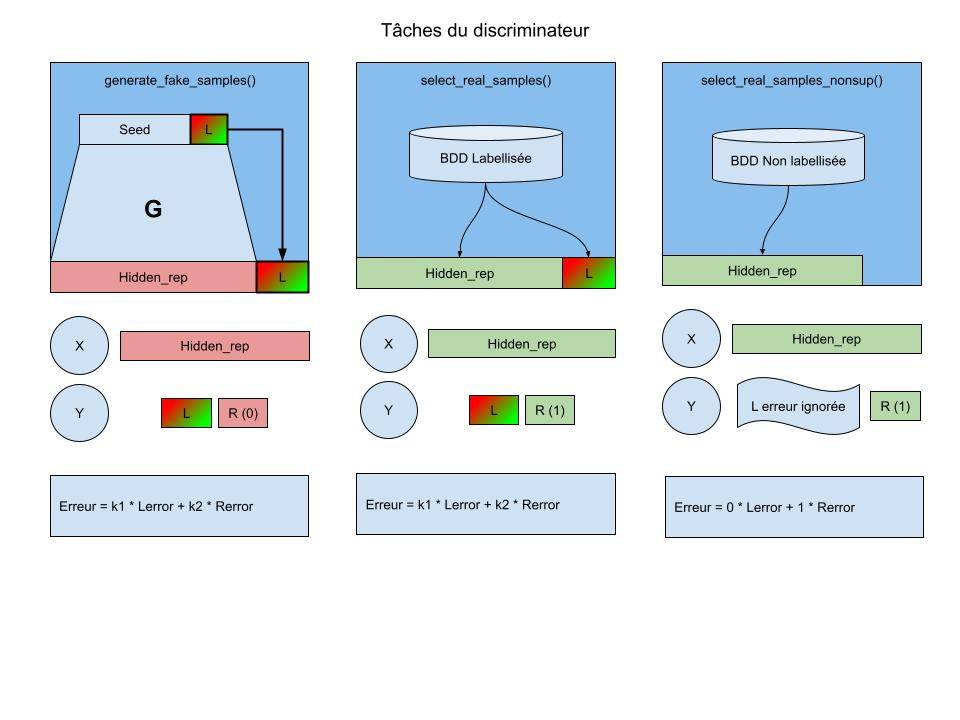
\includegraphics[width=\textwidth]{tacheD.jpg}

	\subsection{GAN}

	Le model advertial est donc l'assembage de G avec D.
	Afin d'entrainer l'architecture il faut alterné l'entainement de G puis de D c'est a dire ne pas effectuer de retropopagation dans D lors de l'entrainement de G et ne pas retropopager dans G lors de l'entrainement de D.
	G est recompensé s'il trompe D sur la realité des donné qu'il generer. Similairement D est recompensé s'il determine quel données sont generé et quel donné ne le sont pas.
	En meme temps la tache de classification du label se fait: (TODO voirsi j'en parle ici)

	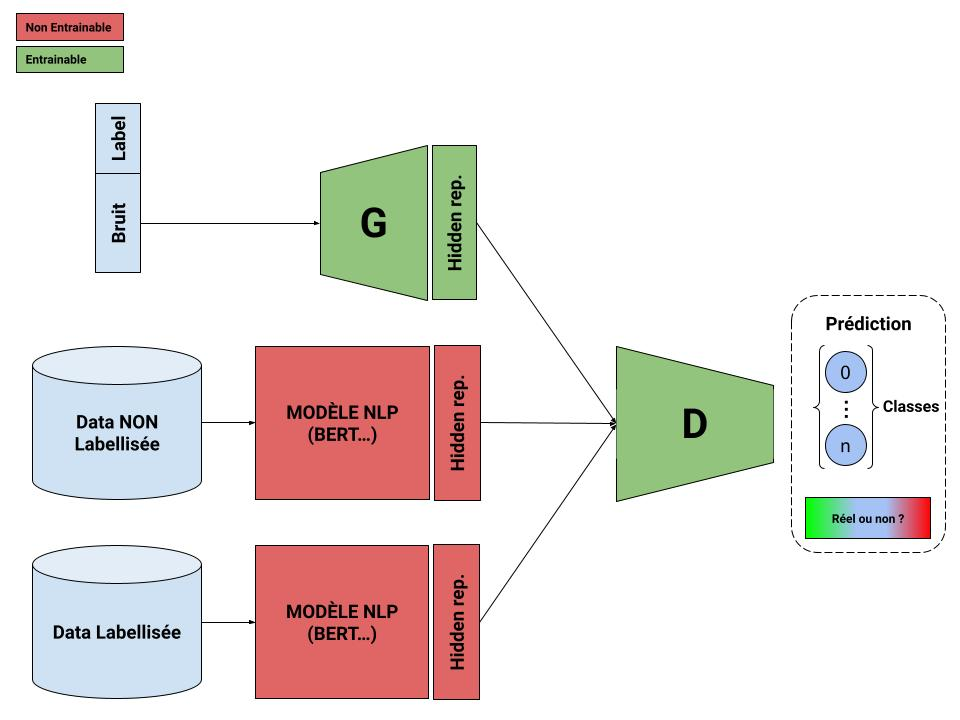
\includegraphics[width=\textwidth]{Architectutre_Entrainement.jpg}

	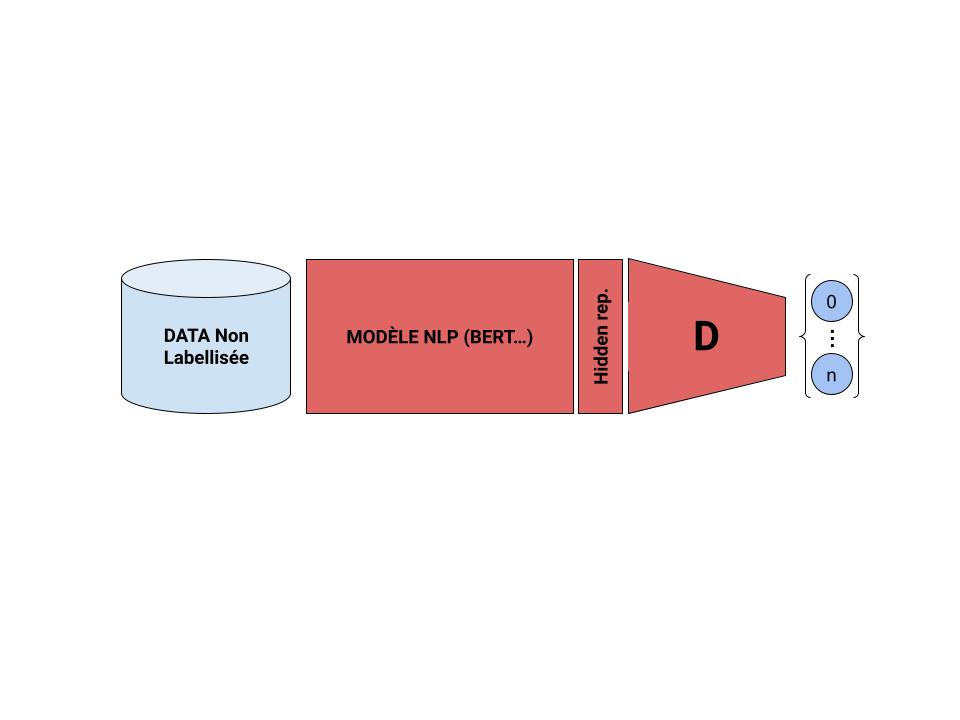
\includegraphics[width=\textwidth]{Architecture_Utilisation.jpg}
	
\section{Entraînement}

	\subsection{Fonctions d'erreurs}
	Comme il s'agit à chaque fois d'une classification binaire c'est l'erreur d'entropie croisée binaire qui est utilisé:
	\[-(y\cdot\log(\hat y) + (1 - y)\cdot\log(1 - \hat y))\]

	Pour le D chacune de ses branches sera evalué avec cette fonction et l'erreur total de la prediction sera la somme des erreurs.
	Comme le G utilise D pour faire ses predictions sont erreur sera calculer comme pour celle du D mais les predictions sont inversé. Ansi G minimise sa fonction d'erreur s'il arrive à tromper D.

	\subsection{Supervisé}

		bce seul sur le label

	\subsection{Semi-supervisé}
		\subsubsection{Competition ou coopération ?}
		\subsubsection{Stabilisation du Générateur et Discriminateur}
\section{Evaluation}
\subsection{Mesures utilisées}
recall, precision, f1 score , APS,AUC
au sein d'une cross validation (5folds, équilibre pour l'entraînement)

\subsection{Comparaison des mesures}
	
\section{Conclusion et perspectives}
perspectives:
generation au niveau des token, utilisation d'un modèle NLP entraîné sur le corpus que l'on souhaite classer 
remplacer la prediction de la realité par une critique comme cela est fait dans un WGAN

test f zjfhizef 
un des probleme de cette architecture est que meme lorsque le generateur n'est pas bon, c'eet a dire qu'il ne genere pas de données proche de la realité, le discriminateur doit quand meme donner un avi et etre penalisé, en depit de la pietre qualité du generateur. pour palier a ce probleme, outre le fait de pourvoire attendre une qualité de generation "satisfaisante" un autre type d'architecture aurais pu etre utilisé comme par exemple les WGAN (TODO citer)

Choie de [CLS] : D'autres (ou combinaison) d'autres representations du model auraient pu etre chosisies.

\end{document}
